\chapter{Algorithmic  composition}

\section{Historical framework}\label{historical-framework}

The first piece of music written by a computer is the \textit{Illiac Suite} for string quartet.

It was realized in 1956 at Illinois University.

Differently from music illustred in previous chapter computer did not generate the waveform but a symbolic representation of musical parameters to be transcribed into a musical score.

\begin{center}
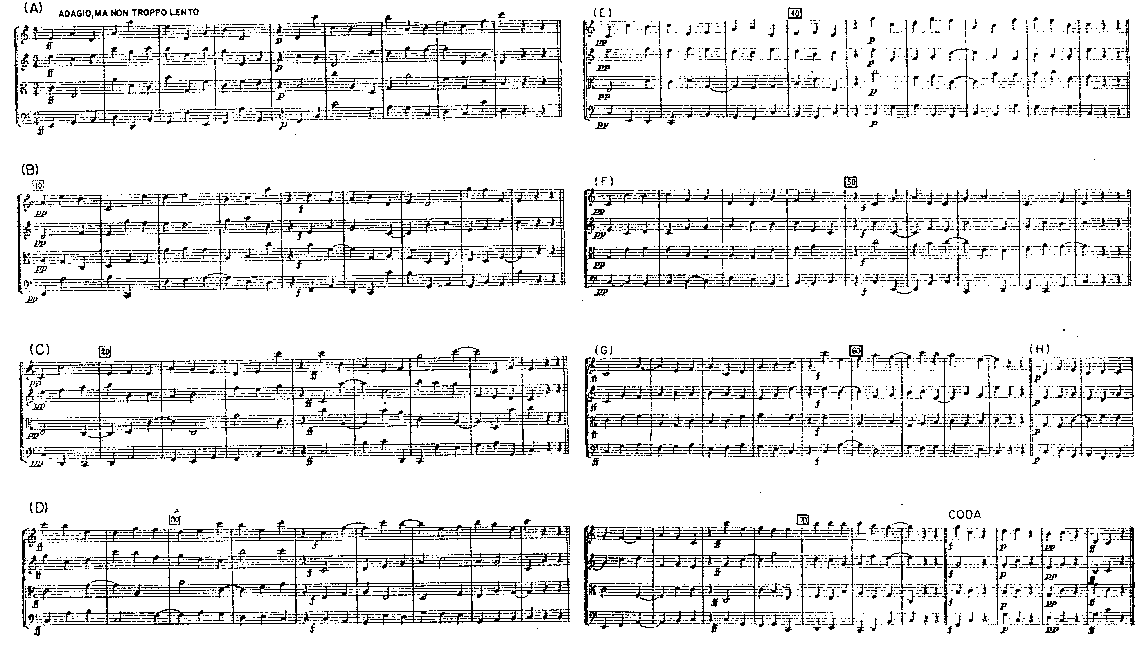
\includegraphics[scale=1]{../img/illiac.png}
\end{center}

This work was an experiment to test various algorithms for composition.

\begin{enumerate}
\def\labelenumi{\arabic{enumi}.}
\tightlist
\item random music \(\rightarrow\) no rules.
\item skip-stepwise rule \(\rightarrow\) no more than one repeated note.
\item cantus firmus starts on C with C chord for opening \(\rightarrow\) cadence on C with leading tone in one of the four voices \(\rightarrow\) resolution f tritone in VII-6, e.g.~F/B must resolve to E/C.
\item octave-range rule.
\item only consonant chords permitted except for 6-4 chords \(\rightarrow\) harmonic subroutine added.
\item parallel unisons, octaves, fifths and fourths still permitted \(\rightarrow\) melodic subroutine added.
\item parallel fourths, 6-4 chords containing tenth still permitted.
\item best counterpoint.
\end{enumerate}

Another important composer in the development of algorithmic music was the greek composer (naturalized french) Iannis Xenakis.

He used formulas developed by scientists to describe the behavior of particles in gases.

He saw his stochastic compositions as clouds of sound with individual notes as the analogue of gas particles organizing in this way clouds of notes.

The choice and distribution of notes was determined by procedures involving random choice, probability tables weighing the occurrence of specific events against those of others.


Iannis Xenakis - \href{http://www.musicaecodice.it/gitmedia/emc/5_media/xen1.mp4}{Pithoprakta} for Orchestra (1955-56) - extract.

Another composer involved in this fields was Gottfried Michael Koenig that worked at the Utrecht University Institute of Sonology and wrote about his Project 1 software:

\textit{Project 1 is based on the findings of serial composition technique, and aims at the experimental experience of chance-governed constellations of parameter values. Chance, in this instance, replaces the permutations to which the serial composer was accustomed to
subjecting rows, the consequences of which action for the resulting constellations of material was scarcely more predictable than in the case of aleatoric manipulations. Just as serial technique soon abandoned the "pointillist" style in order to apply the organizational principle to pre-formed units, "groups", the idea behind Project 1 likewise assumes that the unpredictability of chance will be neutralized by given
lists of material and the appropriate selection of items from the lists, in order to facilitate the formation of medium-sized and larger form categories.}

In more recent times and outside the academic environment a composer like Brian Eno writes:

\textit{Since I have always preferred making plans to executing them, I have
gravitated towards situations and systems that, once set into operation,
could create music with little or no intervention on my part. That is to
say, I tend towards the roles of planner and programmer, and then become
an audience to the results.}

Nowadays it is one of the most explored artistic fields in generative artificial intelligence.

\section{Software installation}\label{software-installation}

In addition to SuperCollider and sc\_kernel (optional) install: 

\begin{itemize}
\tightlist
\item \href{https://lilypond.org/}{Lilypond} 
\item \href{https://github.com/n-armstrong/fosc}{Fosc} (a Supercollider API for generating musical notation in lilypond)
\end{itemize}

Configure Fosc:

\begin{enumerate}
\def\labelenumi{\arabic{enumi}.}
\tightlist
\item download the zip file
\item rename the \textit{fosc-master} folder to \textit{fosc}.
\item select SuperCollider (base) Kernel in this notebook (optional).
\item find your SuperCollider user extension hidden folder path:

\begin{lstlisting}[frame=single] 
Platform.userExtensionDir
\end{lstlisting}

\item move the \textit{fosc} folder to your SuperCollider User Extensions folder.
\item search in SuperCollider Qarks \textit{wslib} and installi it.
\item recompile Class library in SuperCollider or Refresh SuperCollider Kernel in Notebook.
\item add code to allow Fosc to communicate with LilyPond to your sclang startup file.

\pagebreak

Mac users:

\begin{lstlisting}[frame=single] 
this.executeFile("/absolute/path/to/init_mac.scd");
\end{lstlisting}

Windows users:

\begin{lstlisting}[frame=single] 
this.executeFile("/absolute/path/to/init_win.scd");
\end{lstlisting}

\item Test it - generates three files:

\begin{itemize}
\tightlist
\item test.ly
\item test.pdf
\item test.mid
\end{itemize}

We should also hear an audio preview with default intrumental timbre.

\begin{lstlisting}[frame=single] 
~bpm   = 60;
~pitch = [60,64,67,nil,67,64,72,[67,64],nil,64,60,[64,67,72]];
~dur   = [8];
~exp   = [nil];

~print.(~pitch, dur:~dur, vel:~exp, bpm:~bpm);
\end{lstlisting}
\end{enumerate}

We can load the midifile in an external midi sequencer or notation software as Musescore, Garageband, Sibelius, etc.

\section{Symbolic musical representation and numbers}\label{symbolic-musical-representation-and-numbers}

The purpose of this computer music practice is to help the composer generate and manipulate musical elements according to the syntactic rules of their chosen musical language.

One of the goals of algorithmic composition or computer-aided composition is to translate numerical values \hspace{0pt}\hspace{0pt}into symbols specific to musical notation and vice versa.

The final result consists of a musical score that can be interpreted by human performers.

In computer music as well as in western musical tradition the following sound parameters are typically generated and/or manipulated:

\begin{itemize}
\tightlist
\item pitch (frequency).
\item rhythm (time).
\item dynamic (amplitude).
\item expression (timbre).
\end{itemize}

\subsection{Pitch}\label{pitch}

Some symbolic representations of frequency sorted by level of abstraction:

\begin{itemize}
\tightlist
\item Diatonic tones.
  \begin{itemize}
  \tightlist
  \item diatonic representation by letters (notenames) or degrees.
  \item fixed octave.
  \item relative to syntactically defined rules (western music tones, semitones).
  \item typically strings or chars data types.
  \end{itemize}

\begin{lstlisting}[frame=single] 
a = [   0,    1,    2,    3,     4,    5,    6,    7]; // Scale degrees
a = ['do', 're', 'mi', 'fa', 'sol', 'la', 'si', 'do']; // Note name
a = ['C3', 'D3', 'E3', 'F3',  'G3', 'A3', 'B3', 'C4']; // Octave
\end{lstlisting}

\item intervals.

  \begin{itemize}
  \tightlist
  \item determine the pitch relative to a root note (0) in semitones.
  \item no fixed octave.
  \item they may or may not be related to defined syntactic rules (scale degrees or other).
  \item typically int (positive and negative).
  \end{itemize}

\begin{lstlisting}[frame=single] 
a = [ 0, 2, 4, 5, 7, 9, 11, 12]; // Major scale model
a = [-3, 5, 6, -4, 0, 2];        // A sequence 
\end{lstlisting}

\item MIDI note.
  \begin{itemize}
  \tightlist
  \item determines pitch as a fractional MIDI note.
  \item they are not related to syntactically defined rules.
  \item root note \(\rightarrow\) 60 = C4 = middle C.
  \item divided in semitones (int).
  \end{itemize}

\begin{lstlisting}[frame=single] 
a = [ 60, 62, 64, 65, 67, 69, 71, 72];
\end{lstlisting}

\item frequency.
  \begin{itemize}
  \tightlist
  \item determines the pitch as a frequency in Hertz (or cps).
  \item absolute values not relate in any way to syntactically defined rules.
  \item int or float
  \end{itemize}

\begin{lstlisting}[frame=single] 
a = [ 262, 294, 330, 349, 392, 440, 494, 523]; 
\end{lstlisting}
\end{itemize}

In computer music there are further forms of pitch representation but they can easily be traced back to those just mentioned.

In SuperCollider we can convert from a form to another:

\begin{lstlisting}[frame=single] 
~degree    = [0, 2, 4, 5, 7];   // Degree
~root      = 60;
~midinote  = ~root + a;         // Midi note   
~freqency  = ~midinote.midicps; // Frequency
~midinote1 = ~freqency.cpsmidi;
~degree1   = ~midinote1 - 60;

~midinote.postln;               // change
\end{lstlisting}

Chords \(\rightarrow\) 2D arrays.

\begin{lstlisting}[frame=single] 
~pitch = [[60,64,67,72],62,[60,65,69,72],64,[62,65,67,71],62,[60,64,67,72]];
~dur   = 4!6 ++ [2];

~print.(~pitch, ~dur);
\end{lstlisting}

Rest \(\rightarrow\) nil instead note midi number.

\begin{lstlisting}[frame=single] 
~pitch = [60,62,64,nil,65,67,nil,74,73,74,75,nil,76,72,nil,64];
~dur = [16];

~print.(~pitch, ~dur);
\end{lstlisting}

\subsection{Rhythm}\label{rhythm}

We can define any kind of musical event in time choosing at least two of these parameters:

\begin{itemize}
\tightlist
\item onsets \(\rightarrow\) absolute time of a sound event relative to the beginning (as in DAW software).
\item delta times \(\rightarrow\) time between two consecutive sound events.
\item durations \(\rightarrow\) duration of a sound event.
\end{itemize}

All these parameters can be specified as:

\begin{itemize}
\tightlist
\item absolute measurement units (seconds or millisecond).
\item relative to a bpm.

  \begin{itemize}
  \tightlist
  \item 1 \(\rightarrow\) beat, reference unit (could be quarter, eight, whole, etc).
  \item 1/4 \(\rightarrow\) fractional notation.
  \item 0.5 \(\rightarrow\) multiply factor (result from fractional notation).
  \item 3:2 \(\rightarrow\) Rhythmic proportions (ratios of one single beat or its subdivisions).
  \end{itemize}
\end{itemize}

We can convert the values by simple mathematical operations.

\begin{lstlisting}[frame=single] 
~bpm = 82;
~sec = 60/~bpm;  // bpm     --> seconds
~bpm = 60/~sec;  // seconds --> bpm          
\end{lstlisting}

In this chapter we adopt a notation similar to lilypond notation:

\begin{itemize}
\tightlist
\item 1 \(\rightarrow\) whole.
\item 2 \(\rightarrow\) half.
\item 4 \(\rightarrow\) quarter.
\item 8 \(\rightarrow\) eight.
\item 16 \(\rightarrow\) sixteen.
\item 32 \(\rightarrow\) thirty-second.
\item 64 \(\rightarrow\) sixty-fourth.
\end{itemize}

\begin{lstlisting}[frame=single] 
a = [72,76];
b = [16,16,8,32,32,32,32,8,4];

~print.(a, b);
\end{lstlisting}

If we want to define dotted or irregular rhythms we must use this syntax:

\begin{lstlisting}[frame=single] 
//    [unity, [subdivisions] ]
a = [ [4,     [3, 1        ] ] ];
\end{lstlisting}

We can mix regular and irregular/dotted rhythms.

\begin{lstlisting}[frame=single] 
a = [60,     nil,  62,      63,64,nil,[62,66],67,  68, [64,72]];
b = [4,  [4,[3,   1]], [4, [1,  1,  1,     1,  1]], 8, 8];

~print.(a, b);
\end{lstlisting}

\subsection{Dynamic}\label{dynamic}

Three different measurament units:

\begin{itemize}
\tightlist
\item 1.0 \(\rightarrow\) linear amplitude (floating point form 0.0 to 1.0).
\item 127 \(\rightarrow\) midi velocity (integer from 0 to 127).
\item -6 \(\rightarrow\) decibels (from -inf to 0.0).
\end{itemize}

Conversions:

\begin{lstlisting}[frame=single] 
~lin  = 64  / 127;  // velocity to linear
~vel  = 0.5 * 127;  // linear to velocity
~lin1 = -6.dbamp;   // dB to linear
~db   = 0.5.ampdb;  // linear to dB
~cub  = 0.5**4;     // linear to quartic (best for human perception)             
\end{lstlisting}

In this chapter we adopt a mix between amplitude and expression signs because I think that if we want define overall amplitude, crescendo and diminuendos algorithms are not necessary.

Only three velocity levels:

\begin{itemize}
\tightlist
\item nil \(\rightarrow\) mezzoforte.
\item 1-42 \(\rightarrow\) piano.
\item 43-80 \(\rightarrow\) marcato.
\item 81-127 \(\rightarrow\) accentato.
\end{itemize}

\subsection{Collections}\label{collections}

As we saw we can describe sets of values \hspace{0pt}\hspace{0pt}as
collections.

In SuperCollider Array and List.

Collections are a musically neutral data type as they can contain any data type.

In algorithmic composition we can think it musically in two ways:

\begin{itemize}
\tightlist
\item out of time (pre compositional materials).
  \begin{itemize}
  \tightlist
  \item rules paradigm.
  \item item positions on x axis are indexes without time references (scale degree or other).
  \item scale
\begin{lstlisting}[frame=single] 
//          0   1   2   3   4   5   6   7         // Scale degrees
~dorico = [60, 62, 64, 65, 67, 69, 71, 72];       // Absolute pitches
~chrom  = [0, 1, 2, 3, 4, 5, 6, 7, 8, 9, 10, 11]; // Intervals
~dur    = [8];

~print.(~dorico, ~dur);
\end{lstlisting}

  \item series
\begin{lstlisting}[frame=single] 
~serie  = [1, 10, 6, 4, 8, 2, 9, 7, 0, 5, 11, 3]; // Dodecaphony
~reich  = [64, 66, 71, 72, 73, 66];               // Minimalism
~dur    = [8];

~print.(~reich, ~dur);
\end{lstlisting}

  \item harmonic fields (Array or Array 2D)
\begin{lstlisting}[frame=single]
~mayor = [0, 4, 7, 12];
~harm  = [[60, 64, 67, 72], 
          [62, 65, 67, 71], 
          [60, 65, 69,72], 
          [60, 64, 69,72]];
~harmd = [[0, 4, 7, 12],  [2, 5, 7, 11],  [0, 5, 9,12], [0, 4, 9,12]];
~dur   = [8];

~print.(~harm, ~dur);
\end{lstlisting}
  \end{itemize}
  
\item timeline.

  \begin{itemize}
  \tightlist
  \item sequence paradigm.
  \item items are placed on a timeline (x axis).
  \end{itemize}

\begin{lstlisting}[frame=single] 
//   - Sequence of index from defined scale
//          0   1   2   3   4   5   6   7
~scale  = [60, 62, 64, 65, 67, 69, 71, 72];      
~melody = 10.collect({rrand(0,7)});
~seq    = ~melody.collect({arg i; ~scale[i]});               
~dur    = ([16,8,16]!3++[4]).flat; 
~exp    = ~melody.collect({ [nil,100,40].wchoose([0.6,0.2,0.2]) });

~print.(~seq,~dur, ~exp); 
\end{lstlisting}
\end{itemize}

\subsection{Live}\label{live}

Send numerical data via MIDI to external sound generators (Reaktor, GarageBand, Logic) without print it in a musical score.

Open a midi sound generator software and set it.

\begin{lstlisting}[frame=single, caption=Live midi out sender model] 
MIDIClient.init; // Checks available MIDI devices

c = MIDIOut.new(0); // Choose the destination - 0 = "Driver IAC"
c.latency_(0);      // Set latency to 0 sec

~evt   = 100; 
~bpm   = 60;       
~pitch = ~evt.collect({rrand(60,75)});
~durs  = ~evt.collect({[32, 32, 32, 32, 32, 8, 16].choose});
~expr  = ~evt.collect({[100, 40, 60].choose});
p = Pbind(
          \type,     \midi,
          \midicmd,  \noteOn,
          \midiout,  c,
          \chan,     0,
          \midinote, Pseq(~pitch.replace([nil],\rest)),
          \sustain,  Pseq(1/~durs * 4, inf),   // Duration
          \dur,      Pseq(1/~durs * 4,inf),    // Delta time
          \amp,      Pseq(~expr/127,inf),      // 0.0 to 1.0
          ).play;
\end{lstlisting}

\section{Generative techniques and processes}\label{generative-techniques-and-processes}

In western musical tradition superposition of two or more voices have only two approaches: 

\begin{itemize}
\tightlist
\item \href{http://www.musicaecodice.it/gitmedia/emc/5_media/palestrina1.mp4}{counterpoint} (horizontal dimension - static voice allocation).
\item \href{http://www.musicaecodice.it/gitmedia/emc/5_media/beetho1.mp4}{harmony} (vertical dimension - dynamic voice allocation).
\end{itemize}

Approaches to which different musical languages refer.

In general if we want formalize our musical ideas we should act as in previous chapters.

Recap.

\begin{enumerate}
\def\labelenumi{\arabic{enumi}.}
\tightlist
\item choose a set of parametric structures that we want to use as basic material according to musical rules (scale, modes, series, chords, rhythmic or dynamic patterns, etc.).
\item define a set of possible modifications always starting from musical needs and rules (variations, filters, interpolations, augmentations, diminutions, etc.).
\item organize them over time by defining a formal structure choosing from two strategies:
  \begin{itemize}
  \tightlist
  \item top to bottom (from a fixed general structure to particular).
  \item bottom to top (from particular to a general formal structure).
  \end{itemize}
\end{enumerate}

In carrying out these three steps, we have only two possible approaches often mixed toghether:

\begin{itemize}
\tightlist
\item nondeterministic.
\item deterministic.
\end{itemize}

\subsection{Modes and scales}\label{modes-and-scales}

Simplifying:

\begin{itemize}
\tightlist
\item \textit{mode} \(\rightarrow\) gregorian to baroque music. 
\item \textit{scale} \(\rightarrow\) baroque to jazz/pop music.
\end{itemize}
  
The way through which composer organize the pitches of a piece.

They are usually some kind of subdivision of the octave interval.

We can represent it in two ways:

\begin{itemize}
\tightlist
\item intervals \(\rightarrow\) chromatic distance from 0 (root) in semitones.  
\item degrees \(\rightarrow\) diatonic distance from 0 (root) in note names.
\end{itemize}

For exemple major scale:

\begin{lstlisting}[frame=single] 
~degrees   = [0, 1, 2, 3, 4, 5,  6,  7];
~intervals = [0, 2, 4, 5, 7, 9, 11, 12];  
\end{lstlisting}

Then we have to choose a root note in midi values which will assume the function of the first degree (0)

\begin{itemize}
\tightlist
\item in modal rules is called \textit{finalis}.
\item in tonal (harmonic) rules is the \textit{key} (D major, E-flat minor, etc.).
\end{itemize}

\begin{lstlisting}[frame=single] 
~major = [0,2,4,5,7,9,11,12];  
~root  = 60;
~pitch = ~root + ~major;
~dur   = [1/8];
~print.value(~pitch, ~dur, filepath:~filepath); 
\end{lstlisting}

We can use historical models or invent our own.

\subsubsection{Scale}\label{scale}

In SuperCollider there is a repository of different scales from different coltures.

\begin{lstlisting}[frame=single] 
Scale.directory;
\end{lstlisting}

Choose a scale from the availables and recall the interval model.

\begin{lstlisting}[frame=single] 
~model     = Scale.lydian;    
~intervals = ~model.degrees; 
~root      = 60;
~pitch     = ~root + ~intervals;
~dur       = [8];
~intervals,postln;
~pitch.postln;
~print.(~pitch, ~dur); 
\end{lstlisting}

Once the interval model has been established, we can create a melody by recalling the different degrees of the model according to deterministic or indeterministic principles.

\subsubsection{Incises and motives}\label{incises-and-motives}

We can write an incise in a deterministic way.

\begin{lstlisting}[frame=single] 
~mod  = Scale.lydian.degrees;  
~degr = [0,3,nil,5,2,3,6,5]; // in scale degrees
~root = 60;
~ptch = ~degr.collect({arg i; if(i.notNil) {~mod.at(i) + ~root}});
~durs = [8,8,16,16,[8,[1,1,1]],4];
~expr = [nil, 100, nil, nil, nil, nil, nil, 40];
~print.(~ptch, ~durs, ~expr); 
\end{lstlisting}

We can also program a \textit{random incise generator} algorithm. 

It's not necessary but can be a good pratice to formalize algorithm in functions.

This algotithm generate inceses according to simple rules:

\begin{enumerate}
\def\labelenumi{\arabic{enumi}.}
\tightlist
\item set the number of notes.
\item set an interval model. 
\item set a root note.
\item set a percentage of random rests (0.0 - 1.0).

\begin{lstlisting}[frame=single] 
~inc  = {arg evt=1, imodel, root=60, rest=0.0;
         var pitch, rests;
             rests = [imodel,[nil]];      
             pitch = evt.collect{var i; 
                                 i = rests.wchoose([1-rest,rest]).choose;
                                 if(i.notNil)
                                 {i = i + root} }; 
        };
\end{lstlisting}

Test it.

\begin{lstlisting}[frame=single] 
~evt  = rrand(2,5);
~mod  = Scale.lydian.degrees; 
~root = 60;
~rest = 0.2;
~durs = [8];
~seq  = ~inc.(~evt, ~mod, ~root, ~rest);

~print.(~seq, ~durs)
\end{lstlisting}

\item set a database of rhythmic patterns from which to extract one according to the number of pitches. Each pattern should be of the same lenght (a beat or its multiple).

\begin{lstlisting}[frame=single] 
~inc  = {arg evt=1, imodel, root=60, rest=0.0;
         var pitch, rests, durs;
            rests = [imodel,[nil]];      
            pitch = evt.collect{var i; 
                                i = rests.wchoose([1-rest,rest]).choose;
                                if(i.notNil)
                                {i = i + root} }; 
            durs = switch(evt,  
                        2, {[[8,8],
                             [[4,[3,1]]],
                             [[4,[1,3]]],
                             [[4,[2,1]]],
                             [[4,[1,2]]] ].choose},
                        3, {[[8,16,16],
                             [16,8,16],
                             [16,16,8],
                             [[4,[1,1,1]]] ].choose},
                        4, {[[16,16,16,16],
                             [[4,[2,1,1,2]]],   
                             [[4,[2,2,1,1]]]].choose},
                        5, {[[16,16,16,16],
                             [[4,[1,1,1,1,1]]],   
                             [[4,[2,2,1,1,1]]],
                             [[4,[1,2,1,2,1]]]].choose} 
                             );                   
            [pitch, durs] 
        };
\end{lstlisting}

Test it.

\begin{lstlisting}[frame=single] 
~evt  = rrand(2,5);
~mod  = Scale.lydian.degrees;
~root = 60;
~rest = 0.2;
~seq  = ~inc.(~evt, ~mod, ~root, ~rest );

~print.(~seq[0], ~seq[1]);
\end{lstlisting}

\item set a percentage of random velocities/expressions to apply on notes.
   
   2D array:

\begin{itemize}
\tightlist
\item [0] \(\rightarrow\) dataset from wich values are chosen.
\item [1] \(\rightarrow\) percentage of random velocities (0.0-1.0).
\end{itemize}

\begin{lstlisting}[frame=single, caption=random incise function] 
~inc  = {arg evt=1, imodel, root=60, rest=0.0, exp=[[nil],[0.0]];
         var pitch, rests, durs,  vel;
             rests = [imodel,[nil]];    
               
             pitch = evt.collect{var i; 
                                i = rests.wchoose([1-rest,rest]).choose;
                                if(i.notNil)
                                {i = i + root} 
                                };                               

            durs = switch(evt,  
                        2, {[[8,8],
                             [[4,[3,1]]],
                             [[4,[1,3]]],
                             [[4,[2,1]]],
                             [[4,[1,2]]] ].choose},
                        3, {[[8,16,16],
                             [16,8,16],
                             [16,16,8],
                             [[4,[1,1,1]]] ].choose},
                        4, {[[16,16,16,16],
                             [[4,[2,1,1,2]]],   
                             [[4,[2,2,1,1]]]].choose},
                        5, {[[16,16,16,16],
                             [[4,[1,1,1,1,1]]],   
                             [[4,[2,2,1,1,1]]],
                             [[4,[1,2,1,2,1]]]].choose} 
                             );                          
            vel = pitch.collect{arg i;
                                if(i.notNil)
                                {[exp[0],[nil]].wchoose([exp[1],1-exp[1]])
                                               .choose} }.flat;               
            [pitch, durs, vel] 
        };
\end{lstlisting}

Test it.
\begin{lstlisting}[frame=single] 
~evt  = rrand(2,5);
~mod  = Scale.lydian.degrees;
~root = 60;
~rest = 0.2;
~exp  = [[40,100],0.3];
~seq  = ~inc.(~evt, ~mod, ~root, ~rest, ~exp );

~print.(~seq[0], ~seq[1] , ~seq[2]);
\end{lstlisting}
\end{enumerate}

In this way we can also construct motives with several incises.

\begin{lstlisting}[frame=single, caption=random motive function] 
~mot = {arg evt, imodel, root=60, rest=0.0, exp=[[nil],[0.0]];
        var p,r,v;
            p = [];
            r = [];
            v = [];
            evt.do({arg i;
                    i = ~inc.(rrand(2,5), imodel, root, rest, exp);
                    p = p ++ i[0];
                    r = r ++ i[1];
                    v = v ++ i[2]; 
                    });
            [p.flat,r,v.flat]};
\end{lstlisting}

Test it.

\begin{lstlisting}[frame=single] 
~evt  = rrand(3,10);
~mod  = Scale.lydian.degrees;
~root = 60;
~rest = 0.3;
~exp  = [[40,100],0.3];
~seq  = ~mot.(~evt, ~mod, ~root, ~rest, ~exp );
~print.(~seq[0], ~seq[1] , ~seq[2], 
        filepath:'/absolute/path/to/test');
\end{lstlisting}

I'd like to underline:
\begin{itemize}
\tightlist
\item the \textit{~inc} function is based on musical rules we established previously (choice of scale, number of notes, set of rhythmic cells, etc.).
\item in implementing it we mixed deterministic and indeterministic procedures.
\end{itemize}

Now we can save short sequences as single midi files (different names) and edit it in software like Musescore, Sibelius or generic midi sequencer.

\subsubsection{Variations}\label{variations}

In the previous paragraph we generated incises and motives.

Let's see now few possible variations.

Pitches, rhythms and velocities sequencies are represented as Array or List.

In SuperCollider there are numerous methods that we can call on them to modify the contents.

In next exemples we apply methods on specific parameters but in principle almost all methods are valid for all parameters. 

\begin{itemize}
\tightlist
\item chromatic trasposition \(\rightarrow\) sum an offset in semitones (absolute).
    \begin{itemize}
    \tightlist
    \item pitch.
    \end{itemize}

\begin{lstlisting}[frame=single, caption=chromatic transposition function] 
~ctsp = {arg seq=[60], trsp=0;
             seq.collect({arg i; 
                          if(i.notNil) 
                          {trsp + i} 
                          });
         };
\end{lstlisting}

An exemple.

Rules:
\begin{enumerate}
\tightlist
\item define an incise.
\item traspose pitch random +/- 5 semitones n times.
\item duplicate rhythms and velocities n times.
\item put it toghether.
\end{enumerate}

\begin{lstlisting}[frame=single] 
~ptch = [60, 64, 67,  69];
~dur  = [ 8, 16, 16,   8];
~evt  = 3;
~ptch = ~ptch ++ ~evt.collect({ 
                               ~ctsp.(~ptch, rand2(5)) 
                               });
~ptch = ~ptch.flat;
~print.(~ptch, ~dur);
\end{lstlisting}

\item diatonic trasposition \(\rightarrow\) sum an offset in degrees (relative to a scale or interval model).
    \begin{itemize}
    \tightlist
    \item pitch.
    \end{itemize}

\begin{lstlisting}[frame=single, caption=diatonic transposition function] 
~dtsp = {arg seq=[60],trsp=0,scale=[0,2,4,7,9,11];
         var dg;
         seq.collect({arg i, id;
		                  if(i.notNil)
		                  {dg = scale.performKeyToDegree(i, 12);
		                  dg = dg + trsp;
		                  scale.performDegreeToKey(dg,12,0)}
		              })
         };
\end{lstlisting}

An exemple.

\begin{lstlisting}[frame=single] 
~mod  = Scale.major.degrees;
~ptch = [60, 64, 67,  69];
~dur  = [ 8, 16, 16,   8];
~evt  = 3;
~ptch = ~ptch ++ ~evt.collect({ 
                               ~dtsp.(~ptch, rand2(5), ~mod) 
                               });
~ptch = ~ptch.flat;
~print.value(~ptch, ~dur);
\end{lstlisting}

\item retrograde \(\rightarrow\) reverse array items.
    \begin{itemize}
    \tightlist
    \item pitch.
    \item rhythm.
    \item expression.
    \end{itemize}

\begin{lstlisting}[frame=single, caption=retrograde function] 
~retr = {arg seq; seq.reverse};
\end{lstlisting}

An exemple.

Different combinations give different musical results.
\begin{lstlisting}[frame=single] 
~ptch = [60, 67, 76,  nil,72,74,  77];
~dur  = [8,  16, 16,[4,[1, 1, 1]],8];
~exp  = [100, nil, 40, nil, 100, 40,nil];
~ptch  = ~ptch ++ ~retr.(~ptch);
~dur   = ~dur ++ ~retr.(~dur);
~print.(~ptch , ~dur, ~exp);
\end{lstlisting}

\item inversion \(\rightarrow\) hoose a root note for mirroring.
    \begin{itemize}
    \tightlist
    \item pitch.
    \end{itemize}

\begin{lstlisting}[frame=single, caption=inversion function] 
~inv  = {arg seq, root=60;
         seq.collect({arg i;
                      if(i.notNil)
                      {i-root * -1 + root}
                      })
         };
\end{lstlisting}

A deterministic exemple.

Different combinations give different musical results.

\begin{lstlisting}
~ptch = [67, 69, 71,  nil, 65,64];
~dur  = [16];
~exp  = [100, nil, 40, nil, 100, 40,nil];
~root = 73;

~ptch  = ~ptch ++ ~inv.(~ptch, ~root);

~print.(~ptch , ~dur, ~exp);
\end{lstlisting}

\item retrograde of inversion \(\rightarrow\) hoose a root note for mirroring.
    \begin{itemize}
    \tightlist
    \item pitch.
    \end{itemize}

\begin{lstlisting}[frame=single, caption=retrograde of inversion function] 
~rinv = {arg seq, root=60;
             seq = seq.collect({arg i;
                                if(i.notNil)
                                {i-root * -1 + root} 
                                });
             seq.reverse
	     };
\end{lstlisting}

An example that combines different random variations on different parameters.

\begin{lstlisting}
~evt  = 4;        
~ptch = [60,64,67,nil,69,71];
~ptch = [~ptch,                     
         ~retr.(~ptch),
         ~inv.(s, rrand(68,72)),
         ~rinv.(s, rrand(68,72))];
         
~dur = [8,16,16,8,8,16,16,8];
~dur = [~dur, ~retr.(~dur)];

~exp = [100, nil, 40, nil, 100, 40];

~ptch = (~evt.collect({~ptch.choose})).flat;   
~dur  = (~evt.collect({~dur.choose})).flatten(1);

~print.(~ptch, ~dur, ~exp);
\end{lstlisting}

\item palindrome without last element \(\rightarrow\) there are different versions for different musical situations, see Array help file.
    \begin{itemize}
    \tightlist
    \item pitch.
    \item rhythm.
    \item expression.
    \end{itemize}

\begin{lstlisting}[frame=single, caption=palindrome function] 
~pal = {arg seq; seq.mirror1};
\end{lstlisting}

As exemple a radom palindrome plus random diatonic trasposition.

\begin{lstlisting}
~evt  = 10;
~mod  = Scale.major.degrees;
~ptch = [60,64,67,69];
~ptch = [~pal.(~ptch), ~ptch]; 
~ptch = ~evt.collect({ ~dtsp.(~ptch.choose, rand2(3), ~mod) });
~ptch = ~ptch.flat;
~dur  = [32];
~exp  = [100, nil, nil,nil,nil,nil];

~print.(~ptch, ~dur,~exp);
\end{lstlisting}

\item stretching \(\rightarrow\) re-scale rhythms by a scaling factor (multiples of 2).
    \begin{itemize}
    \tightlist
    \item rhythm.
    \end{itemize}

\begin{lstlisting}[frame=single] 
~evt  = 3; 
~ptch  = [60,64,67,nil,69,71,74,67];
~dur   = [8,16,16,16,16,8];
~scale = [0.5,1,2];         
~dur   = (~evt.collect({ 
                        (~dur * ~scale.choose).asInteger
                        })
          ).flatten(1);

~print.value(~ptch, ~dur);
\end{lstlisting}

\item permutation \(\rightarrow\) all possible (array size max 170 items).
    \begin{itemize}
    \tightlist
    \item pitch.
    \item rhythm.
    \item expression.
    \end{itemize}

\begin{lstlisting}[frame=single, caption=all permutations function] 
~perm = {arg seq;
	     var evt;
	         evt = seq.size.factorial.postln;
	         evt.collect({arg i;
		                  seq.permute(i) 
		                  })
         }
\end{lstlisting}

As exemple we can apply it on irregular rhytmic subdivisions.

\begin{lstlisting}
~evt  = 5;                    
~ptch = [60,67,nil,76,72,83, 53,nil,55];
~ptch = ~perm.(~ptch).postln; 
~ptch = ~evt.collect({~ptch.choose}).flat;

~subd = [1,2,1,1];            
~prms = ~perm.(~subd).postln; 
~dur  = ~evt.collect({[[4,~prms.choose],4]}).flatten(1);

~exp = [100, nil, 30,nil,nil,nil];

~print.(~ptch, ~dur, ~exp);
\end{lstlisting}

\item random order. \(\rightarrow\) change order in random way.
    \begin{itemize}
    \tightlist
    \item pitch.
    \item rhythm.
    \item expression.
    \end{itemize}

\begin{lstlisting}[frame=single, caption=random order function] 
~rordr = {arg seq; seq.scramble};
\end{lstlisting}

A randomic variation of previous exemple.

\begin{lstlisting}
~evt  = 5;                // repetitions
~subd = [1,2,1,1];        // subdivision
~ptch = [60,67,nil,76,72,83, 53,nil,55];
~ptch = ~evt.collect({~rordr.(~ptch)}).flat;
~dur  = ~evt.collect({[4,[4,~rordr.(~subd)]]}).flatten(1);
~exp  = [100, nil, 30,nil,nil,nil];
~print.(~ptch, ~dur, ~expr);
\end{lstlisting}

This is an example of when deterministic and indeterministic procedures achieve the same perceptual result.

This happens when deterministic procedures provide too many similar variations making them indistinguishable from each other.

As can be intuited from some of the examples the most musically interesting results are obtained by combining different variation techniques. 

It's true for a single parameter and in the combination of different parameters.

\item phasing. \(\rightarrow\) use arrays of different lengths for the parameters.
    \begin{itemize}
    \tightlist
    \item pitch.
    \item rhythm.
    \item expression.
    \end{itemize}
    Replace the .at() method with .wrapAt() or foldAt().

    Look at Array help files what they do.

\begin{lstlisting}[frame=single] 
~evt  = 40;
~ptch = [60, 75, nil, 76, 79, 92, nil, 70];
~rhyt = [ 8, 16,  16, 16,  8, 4];
~exp  = [80, nil, nil,nil, nil,  30, nil, nil, nil];
~ptch = ~evt.collect({arg i; ~ptch.wrapAt(i)}).flat;
~rseq = ~evt.collect({arg i; ~rhyt.foldAt(i)}).flatten(1);
~vseq = ~evt.collect({arg i; ~acc.wrapAt(i)}).flat;

~print.(~ptch, ~rseq, ~exp);
\end{lstlisting}
\end{itemize} 

In the Array help file we can find further examples of operations on sequences of symbols that can easily be applied to parameters taken into consideration.

\subsection{Harmonic fields}\label{harmonic-fields}

In harmonic systems the interval patterns that define the type of chord are built on the degrees of a scale:

\begin{itemize}
\tightlist
\item tonica \(\rightarrow\) I degree. 
\item mediante \(\rightarrow\) III degree.
\item dominante \(\rightarrow\) V degree.
\item etc.
\end{itemize}

\begin{lstlisting}[frame=single] 
// degree   I       II      III      IV       V         VI        VII
~triadi = [[0,4,7],[2,5,9],[4,7,11],[5,9,12],[7,11,14],[9,12,16],[11,14,17]];
~root   = 60;
~print.(~triadi + ~root,[2])
\end{lstlisting}

The basic chords are made up of three notes \(\rightarrow\) triads. 

In many harmonic systems one of them is doubled \(\rightarrow\) four notes.

There are also chords made up of four or more notes without doubling (seventh, ninth, eleventh and thirteenth chords).

\begin{lstlisting}[frame=single] 
~settime = [[0,4,7,11],[2,5,9,12],[4,7,11,14],[5,9,12,16],
            [7,11,14,17],[9,12,16,19],[11,14,17,21]];
~root    = 60;
~print.(~settime + ~root,[2])
\end{lstlisting}

\subsubsection{Chord database}\label{chord-database}

We define the function \textit{~chord} which contains a database of interval patterns of the language we want to use.

To allow for the use of seventh chords and to even out the voicing we use four-note chords.

Arguments:
\begin{itemize}
\tightlist
\item root note.
\item chord sigle.
\end{itemize}

Output \(\rightarrow\) array of midi notes obtained by mapping the acronym to the corresponding interval pattern.

\begin{lstlisting}[frame=single, caption=chord model function] 
~chord = {arg root, type;
          var intv;
              intv = (maj:    [0, 4, 7, 12],
                      maj7:   [0, 4, 7, 11],
                      maj6:   [0, 4, 7,  9],
                      maj9:   [0, 4, 7, 14],
                      min:    [0, 3, 7, 12],
                      min7:   [0, 3, 7, 10],
                      min6:   [0, 4, 7, 9],
                      min9:   [0, 3, 7, 14],
                      dom7:   [0, 4, 7, 10],
                      dom9:   [0, 4, 7, 14],
                      ecc:    [0, 4, 8, 12],
                      dim:    [0, 3, 6, 12],
                      dim7:   [0, 3, 6, 9]
                      )[type];
          intv.collect({arg i; root + i});
          };
\end{lstlisting}

Choose a chord sigle and a root note.

\begin{lstlisting}[frame=single] 
~ptch = ~chord.(60, \min9);
~print.([~ptch], [2]);
\end{lstlisting}

We can apply a chord pattern to all degrees of a scale, creating an harmonic progression.

\begin{lstlisting}[frame=single] 
~progClassic = [~chord.(60, \maj),
                ~chord.(64, \min),
                ~chord.(67, \dom7),
                ~chord.(69, \min7),
                ~chord.(62, \dom7),
                ~chord.(67, \dom7),
                ~chord.(60, \min),
                ~chord.(65, \dom7),
                ~chord.(58, \maj),
                ~chord.(71, \dim),
                ~chord.(72, \maj),
                ~chord.(60, \maj),
                ];
~print.(~progClassic, [4]);
\end{lstlisting}

A little more Jazzy.

\begin{lstlisting}[frame=single] 
~progJazzy=[~chord.(60, \maj7),
            ~chord.(65, \maj6),
            ~chord.(68, \min7),
            ~chord.(67, \dom7),
            ~chord.(73, \min6),
            ~chord.(68, \maj7),
            ~chord.(60, \min9),
            ~chord.(63, \maj6),
            ~chord.(57, \dim),
            ~chord.(54, \maj9),
            ~chord.(63, \min),        
            ~chord.(60, \maj7),
            ];              
~print.(~progJazzy, [4]);
\end{lstlisting}

\subsubsection{Voicing}\label{voicing}

In the previous sequences all chords are presented in close voicing form.

Intervals between the highest and lowest notes is relatively small, usually within an octave.

All chords can also assume the open voicing configuration.

Intervals are spanned over multiple octaves.

We change the shape of a chord from close to open voicing form.

\begin{lstlisting}[frame=single, caption=voicing model function] 
~voicing = {arg note=[60,64,67,72], octave = [-1,0,-1,0];
                note.collect({arg note, i; octave[i]*12 + note}) };
\end{lstlisting}

Test it.

\begin{lstlisting}[frame=single] 
~closed = ~chord.(60, \maj);                 
~open   = ~voicing.(~closed, [-1,0,-1,0]); 
~print.([~closed, ~open],[2])
\end{lstlisting}

In both forms chords are in the root state and proceed in parallel motion.

In classical harmony, a chord can be represented in an inversion.

Inversions are obtained by transposing one of the chord's notes up an octave.

In a three-note chord there are three possible inversions, in a four-note chord four, and so on.

We can use the same function.

\begin{lstlisting}[frame=single] 
~fond   = ~chord.(60, \maj);                 
~first  = ~voicing.(~fond, [1,0,0,0]); 
~second = ~voicing.(~fond, [1,1,0,0]); 
~print.([~fond, ~first, ~second],[2])
\end{lstlisting}

In pop and jazz, there are various techniques for creating inversions.

The most commonly used are:

\begin{itemize}
\tightlist
\item drop 2 \(\rightarrow\) transpose one octave below the second note from the top.
\item drop 3 \(\rightarrow\) transpose one octave below the third note from the top.
\end{itemize}

Chords in these forms appear fuller and more rounded than their root form.

These techniques combine the concepts of inversion and close-open voicing.

Let's define two functions that realize them.

\begin{lstlisting}[frame=single, caption=drop model functions] 
~drop2={arg chord;
        var sorted, dropNote,newVoicing; 
            sorted        = chord.sort;
            dropNote      = sorted[2];    // 2nd highest
            newVoicing    = sorted.copy;
            newVoicing[2] = dropNote - 12;
            newVoicing.sort 
        };
~drop3={arg chord;
        var sorted, dropNote,newVoicing; 
            sorted        = chord.sort;
            dropNote      = sorted[1]; // 3rd highest
            newVoicing    = sorted.copy;
            newVoicing[1] = dropNote - 12;
            newVoicing.sort 
        };
\end{lstlisting}

Test it.

\begin{lstlisting}[frame=single] 
~fond = ~chord.(72, \maj6);
~d2   = ~drop2.(~fond);
~d3   = ~drop3.(~fond);
~print.([~fond,~d2,~d3], [2])
\end{lstlisting}

These two techniques work well with typical jazz harmonies, but they don't work with classical harmonic progressions because they keep the voices moving in parallel.

Let's transform the previous jazzy progression into late parts (drop 3).

\begin{lstlisting}[frame=single] 
~prog = ~progJazzy.collect({arg i; ~drop3.(i)});             
~print.(~prog, [4]);
\end{lstlisting}

Make a progression more dynamic by randomly choosing the shape of each chord.

\begin{lstlisting}[frame=single] 
~prog = ~progJazzy.collect({arg i;
                                d = rand(3);
                                switch(d,
                                       0, {i},
                                       1, {~drop2.(i)},
                                       2, {~drop3.(i)}) });
~print.(~prog, [4]);
\end{lstlisting}

\subsubsection{Voice-leading}\label{voice-leading}

Voice leading seeks to:

\begin{itemize}
\tightlist
\item minimize pitch distance between successive notes in each voice.
\item preserve common tones (same note between chords).
\item avoid big leaps (> octave) unless musically justified.
\item maintain a consistent order: low → high (no voice crossing).
\end{itemize}

Let's define a function that realizes it between two chords.

\begin{lstlisting}[frame=single, caption=voice-leading model function] 
~vLead = {arg ch1, ch2;
          var result, octVar;
              result = List.new;
              octVar = {arg note; [note - 12, note, note + 12]};
              ch2.do({arg note, i;
                      var cand, best;
                          cand = octVar.(note);
                          best = cand.sortMap({arg n; (n - ch1[i]).abs}).first;
                      result.add(best) });
              result };
\end{lstlisting}

Test it.

\begin{lstlisting}[frame=single] 
a = [~chord.(60, \maj7), ~chord.(71, \maj6)];
b = ~vLead.(a[0],a[1]);
~print.(a++[a[0]]++[b],[2]);
\end{lstlisting}

Let's apply the function to a chords sequence.

\begin{lstlisting}[frame=single] 
~prevSeq   = ~progJazzy;            // Starting sequence
~prevChord = ~prevSeq[0];           // First chord (midi notes)
~voicedSeq = [~prevChord];          // Put it in final sequence
~prevSeq.drop(1).do({arg nextChord; // Start from second chord
                     var voiced;                           
                         voiced     = ~vLead.(~prevChord, nextChord); 
                         ~voicedSeq = ~voicedSeq.add(voiced); 
                         ~prevChord = voiced });
~print.(~prevSeq ++ ~voicedSeq,[4]);
\end{lstlisting}

The algorithm just described works well with jazz and pop harmonies but is less effective when applying traditional harmony rules. We add a function that searches for common notes.

\begin{lstlisting}[frame=single, caption=voice-leading common notes model function] 
~vLeadC= {arg ch1, ch2;
          var result, remain, octVar;
              result = List.new;
              remain = ch2.copy;
              octVar = {arg note; [note-12, note, note+12]};
          ch1.do({arg note1; 
                  var intv, common;
                      intv   = note1 % 12;
                      common = remain.detect({arg n; (n % 12) == intv});
                      if(common.notNil)
                      {result.add(common);
                       remain = remain.reject({arg n; n == common})} });
          ch1.do({arg note1; 
                  var best, cand, baseNote, octaveShift;
                  if(result.collect({arg n; n%12}).includes(note1%12)==false) 
                      {cand = remain.collect({arg n; octVar.(n)}).flat;
                       cand = cand.sortMap({arg cand; (cand - note1).abs});
                       best = cand.detect({arg cand;
                       remain.includes(cand%12 + (cand-(cand%12))) || true});
                       best = cand.first;
                       baseNote = remain.detect({arg n; (n%12)==(best%12) });
                       octaveShift = best - baseNote;
                       result.add(baseNote + octaveShift);
                       remain = remain.reject({arg n; n == baseNote });
                       } });
          result };
\end{lstlisting}

Test it.

\begin{lstlisting}[frame=single] 
a = [~chord.(60, \maj7), ~chord.(71, \maj6)];
b = ~vLeadC.(a[0],a[1]);

~print.(a++[a[0]]++[b],[2]);
\end{lstlisting}

Test it with a chords sequence.

\begin{lstlisting}[frame=single] 
~prevSeq   = ~progClassic.collect({arg i;  ~voicing.(i, [-1,0,-1,0])}); 
~prevChord = ~prevSeq[0];       // First chord (midi notes)
~voicedSeq = [~prevChord];      // Put it in final sequence

~prevSeq.drop(1).do({arg nextChord; // Start from second chord
                    var voiced     = ~vLeadC.(~prevChord, nextChord); 
                        ~voicedSeq = ~voicedSeq.add(voiced);         
                        ~prevChord = voiced });
~print.(~prevSeq ++ ~voicedSeq,[4]);
\end{lstlisting}

By applying voicing, dropping, and voice-leading, we can generate variations in chord sequences while maintaining musical coherence and unity.

We can apply rhythms and all the variations illustrated above.

\begin{lstlisting}[frame=single] 
~prevSeq   = ~progJazzy.collect({arg i;  ~drop3.(i)}); 
~prevChord = ~prevSeq[0];      
~voicedSeq = [~prevChord];      

~prevSeq.drop(1).do({arg nextChord; 
                     var voiced     = ~vLeadC.(~prevChord, nextChord); 
                         ~voicedSeq = ~voicedSeq.add(voiced);         
                         ~prevChord = voiced });
~rhythm = [4,16,8,16,8,8,4,4];
~print.(~prevSeq ++ ~voicedSeq,~rhythm);<<<
\end{lstlisting}

An example of further variations in the construction of a chord sequence can be represented by the use of a random-walk.

\begin{lstlisting}[frame=single, caption=chord random walk model function] 
~chWalk = {arg chords, n=10;
           var idx = 0;
               n.collect({var ch, walk;               
                              ch   = chords[idx];
                              walk = [ -1, 0, 1 ].wchoose([0.4, 0.2, 0.4])
                                                 .clip(0, chords.size-1);
                              idx  = idx + walk;
                              ch }) };
~voicedSeq = ~chWalk.(~progJazzy,25);
~rhy       = 10.collect({[16,8,16].scramble}).flat;
~print.(~voicedSeq,~rhy);
\end{lstlisting}

\subsubsection{Melodies}\label{melodies}

In harmonic systems, melodic lines are based on chord progressions.

We must somehow "extract" a possible melody from a defined chord sequence.

To do this automatically, we can use various algorithms.

Once we have obtained the monodic arrays we can apply all the techniques illustrated previously for any kind of variations.

\paragraph{Top note}\label{top-note}
The simplest.

\begin{lstlisting}[frame=single, caption=top note melody model function] 
~meloTop = ~progJazzy.collect({arg chord; chord.maxItem});
~exp     = [120, nil, nil,100, nil,  30, nil, nil, nil].scramble;
~print.(~meloTop++~progJazzy,[16],~exp);
\end{lstlisting}

\paragraph{Random note}\label{random-note}
The classic.

\begin{lstlisting}[frame=single, caption=random note melody model function] 
~meloRand = ~progJazzy.collect({arg chord; chord.choose});
~exp      = [120, nil, nil,100, nil,  30, nil, nil, nil];
~print.(~meloRand++~progJazzy,[16],~exp);
\end{lstlisting}

\paragraph{Arpeggiating note}\label{arpeggiating-note}
The complete.

\begin{lstlisting}[frame=single, caption=arpeggiating note melody model function] 
~meloArp = ~progJazzy.collect({arg chord; chord.scramble}).flat; 
~exp     = [120, nil, nil,100, nil,  30, nil, nil, nil];
~print.(~meloArp++~progJazzy,[16],~exp, 96);
\end{lstlisting}

\paragraph{Voice-leading style}\label{Voice-leading-style}
A version that tries to move by small intervals into the next chord.

\begin{lstlisting}[frame=single, caption=voice-leading style melody model function] 
~vLeadMel = {arg chord, n = 10;
             var lastNote = 60, nextNote;               
                 nextNote = chord.sort
                                 .minItem({arg n; (n-lastNote).abs});
                 lastNote = nextNote };
~melo = ~progJazzy.collect({arg ch; ~vLeadMel.(ch, ~noteForChord)}).flat;
~rhy  = 3.collect({[16,8,16].scramble}).flat;
~exp  = [120, nil, nil,100, nil,  30, nil, nil, nil].scramble;
~print.(~melo++~progJazzy,~rhy,~exp);
\end{lstlisting}

Adding probabilistic movement around the “closest” tone.

It doesn’t always take the strict nearest note creating more variations.

\begin{lstlisting}[frame=single, caption=voice-leading 2 style melody model function] 
~vLeadMel2 = {arg chord, n = 10;
              var lastNote = 60, nextNote;
                  if(0.8.coin) 
                  {nextNote = chord.sort
                                   .minItem({arg n; (n-lastNote).abs})} 
                  {nextNote = chord.choose};
                  lastNote = nextNote };
~melo = ~progJazzy.collect({arg ch; ~vLeadMel2.(ch, ~noteForChord) }).flat;
~rhy  = 3.collect({[16,8,16].scramble}).flat;
~exp  = [120, nil, nil,100, nil,  30, nil, nil, nil].scramble;
~print.(~melo++~progJazzy,~rhy,~exp, 80);
\end{lstlisting}

Passing notes between chords

If you want it to “walk” through stepwise notes between chord changes instead of jumping only to chord tones you can interpolate.

\begin{lstlisting}[frame=single, caption=melodic-walk style model function] 
~melodyWalk = {arg chords, n = 10;
               var lastNote, idx;
                   lastNote = 60;
                   idx = 0;

    n.collect({var chord, nextChordNote,step,nextNote;
                chord = chords[idx];  
                nextChordNote = chord.sort.minItem({arg n; (n-lastNote).abs});
                step = (nextChordNote - lastNote).sign;
                nextNote = if((lastNote != nextChordNote) and: {0.7.coin}) 
                             {lastNote + step }  // take step
                             {nextChordNote};
                lastNote = nextNote;
                idx = (idx + 1) % chords.size;
                nextNote })
               };
~prevSeq = ~progClassic.collect({arg i;  ~drop3.(i)}); // Starting sequence
~melo    = ~melodyWalk.(~prevSeq);
~rhy     = 3.collect({[16,8,16,4].scramble}).flat;
~exp     = [120, nil, nil,100, nil,  30, nil, nil, nil].scramble;
~print.(~melo++~prevSeq,~rhy,~exp, 52);
\end{lstlisting}

\section{Composition sketches proposal}\label{composition-sketches-proposal}

\begin{enumerate}
\def\labelenumi{\arabic{enumi}.}
\tightlist
\item sketch a formal scheme  (A B A or other) divided into sections and measures.
\item define a basic chord sequence (theme).
\item create a database of variations of the basic sequence, saving them as MIDI files.
    \begin{itemize}
    \tightlist
    \item diversify the vocal lines.
    \item apply variations.
    \item transpose it.
    \end{itemize}
\item assemble the individual files in scoring software (MuseScore, Sibelius, or other) or in a MIDI sequencer according to the formal scheme in point 1.
\item extract melodies from the harmonic scheme and, if necessary, create melodic variations.
\item assemble everything in scoring software or sequencers to create the complete score.
\end{enumerate}

Remember that chords can be tonal, a-tonal, jazzy, spectral, randomic, dodecaphonic, etc.